En esta sección se resolverán 2 problemas relacionados con \textit{string matching} usando el
algoritmo KMP y la función de error de la que se habló en el capítulo 4. Se resolverán los
problemas usando C++ y Haskell y se compararán ambas versiones.

\section{SPOJ}
SPOJ (Sphere Online Judge)
% https://wiki.haskell.org/SPOJ
% Tomar algo del competitive aquí

\subsection{Encontrar el factor de repetición de una cadena}
Recordemos en el capítulo 3 \hyperlink{repetition_factor}{el problema 32.1}, es aquí cuando lo
bonito de la programación competitiva y resolver ejercicios se juntan. Ése problema es lo mismo
a resolver lo siguiente y aún mejor, en un juez en línea que puede ``probar'' la implementación.
La especificación del problema dice lo siguiente: 
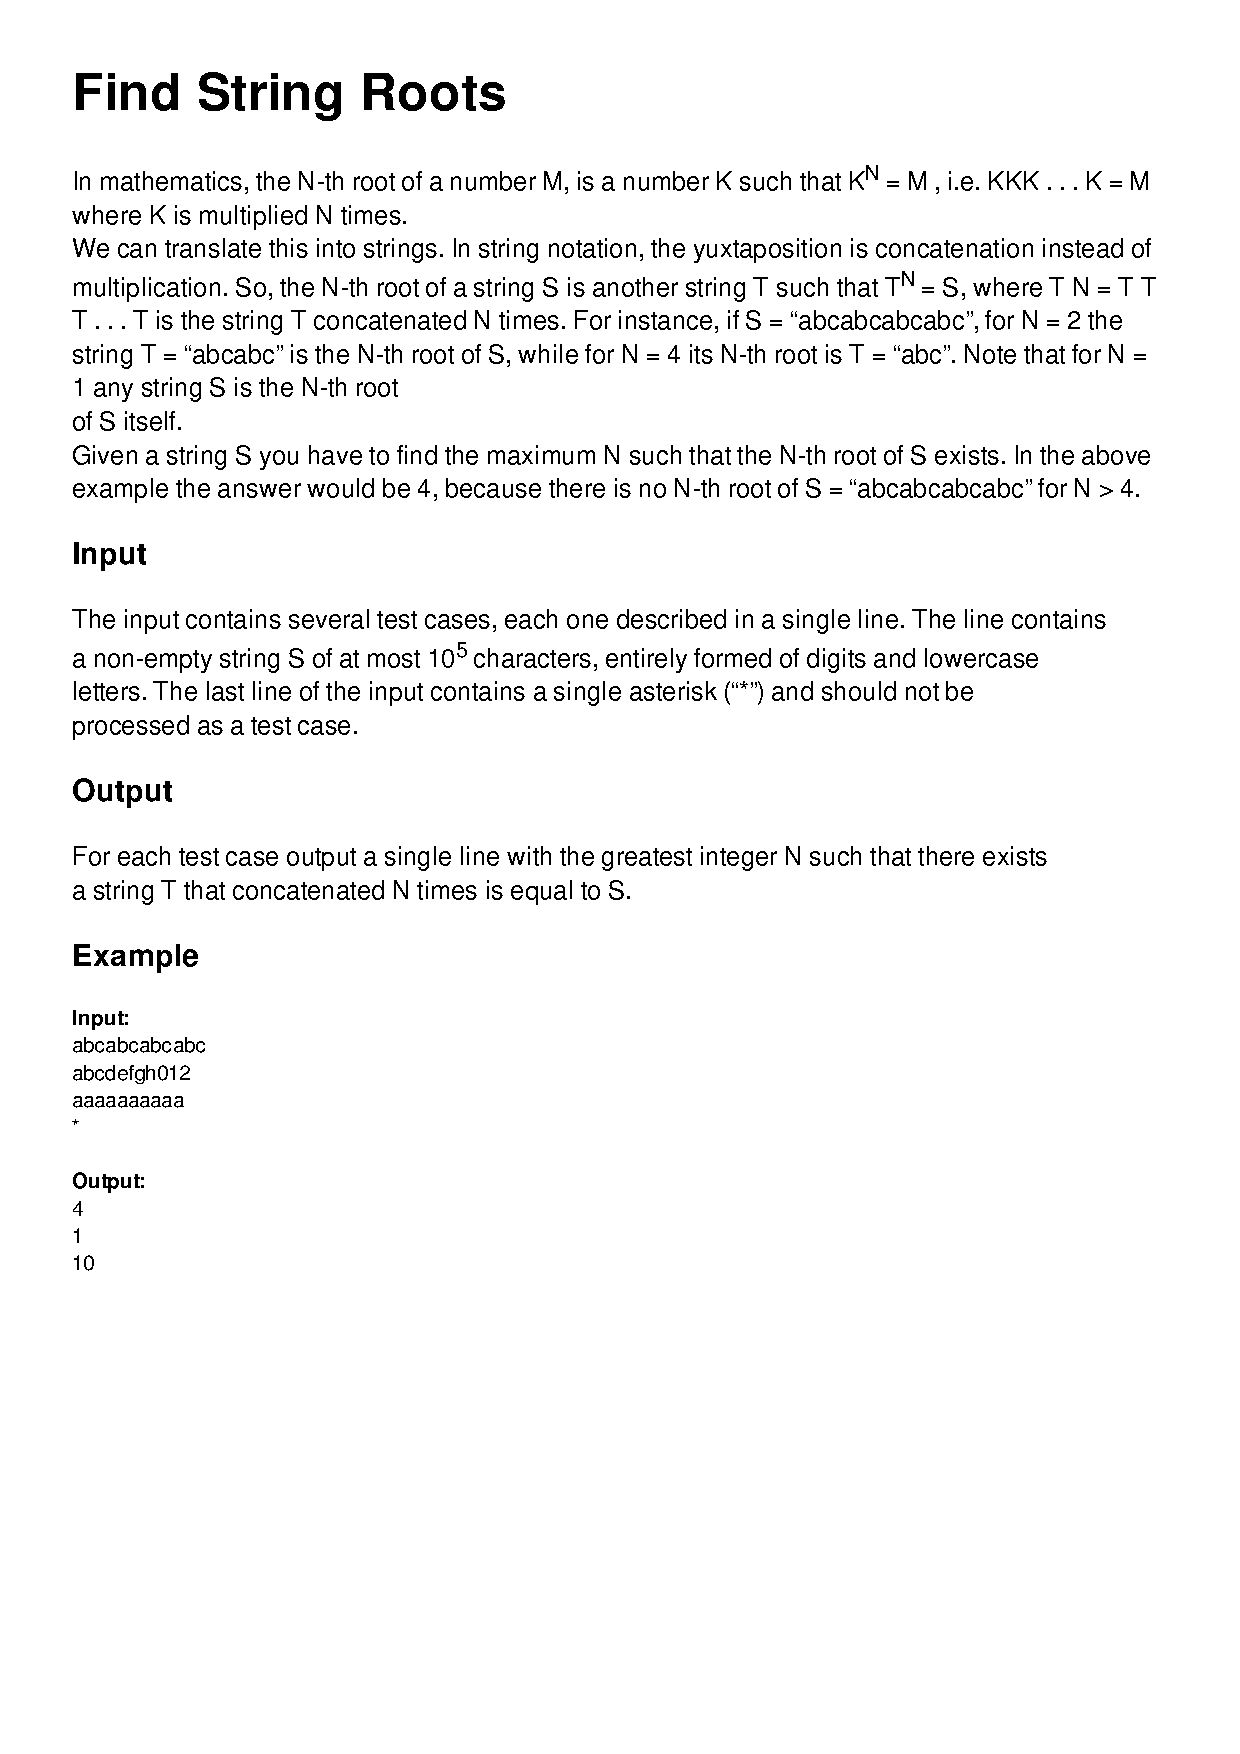
\includepdf[pages=-]{problemas/pdf/FINDSR.pdf}

\inputminted[linenos, frame=lines]{cpp}{problemas/cpp/FINDSR.cpp}
\pagebreak

\inputminted[linenos, frame=lines]{haskell}{problemas/haskell/FINDSR.hs}
\pagebreak

\subsection{Ver si una cadena es una rotación cíclica de otra}
\hyperlink{cyclic_rotation}{el problema 32.4-7}
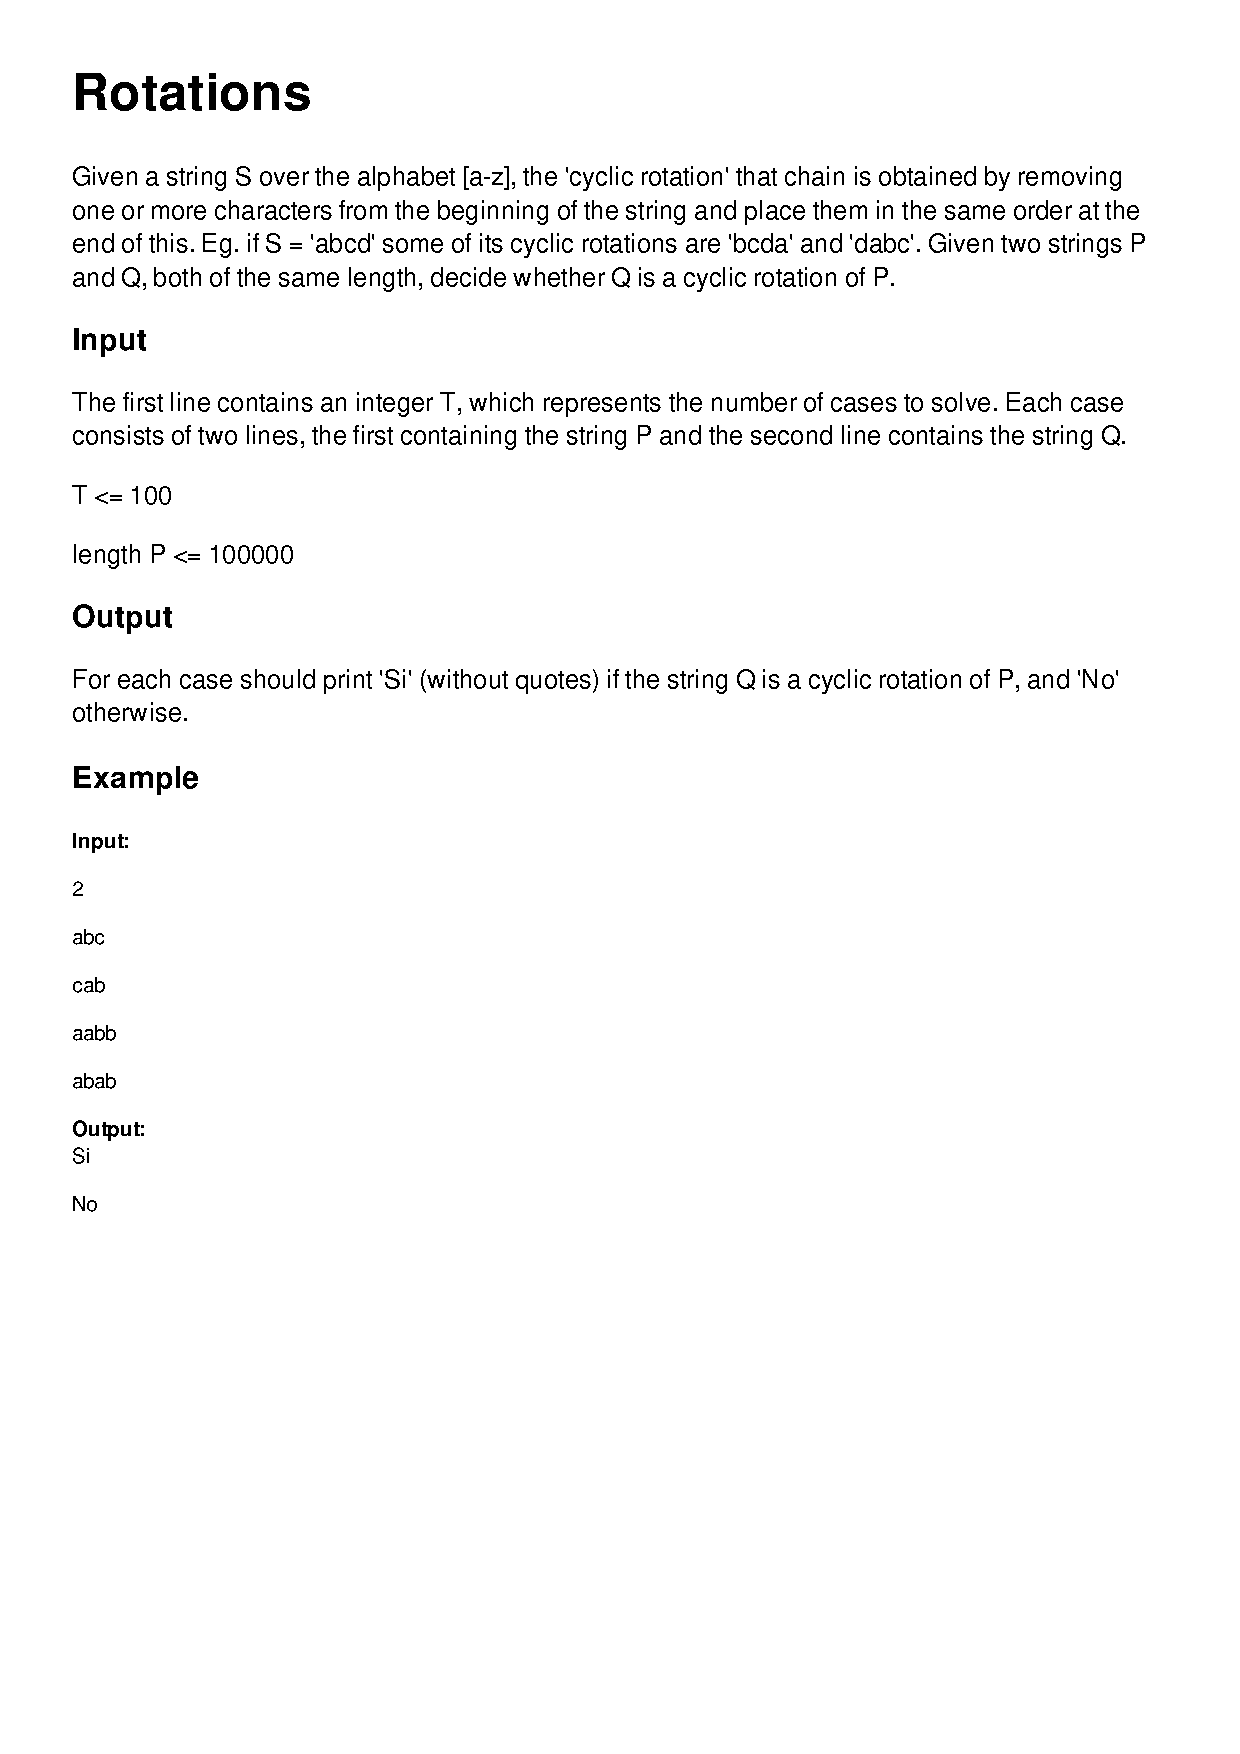
\includepdf[pages=-]{problemas/pdf/EC_WORLD.pdf}

\inputminted[linenos, frame=lines]{cpp}{problemas/cpp/EC_WORLD.cpp}
\pagebreak

\inputminted[linenos, frame=lines]{haskell}{problemas/haskell/EC_WORLD.hs}
\pagebreak

\subsection{Extender el palíndromo}
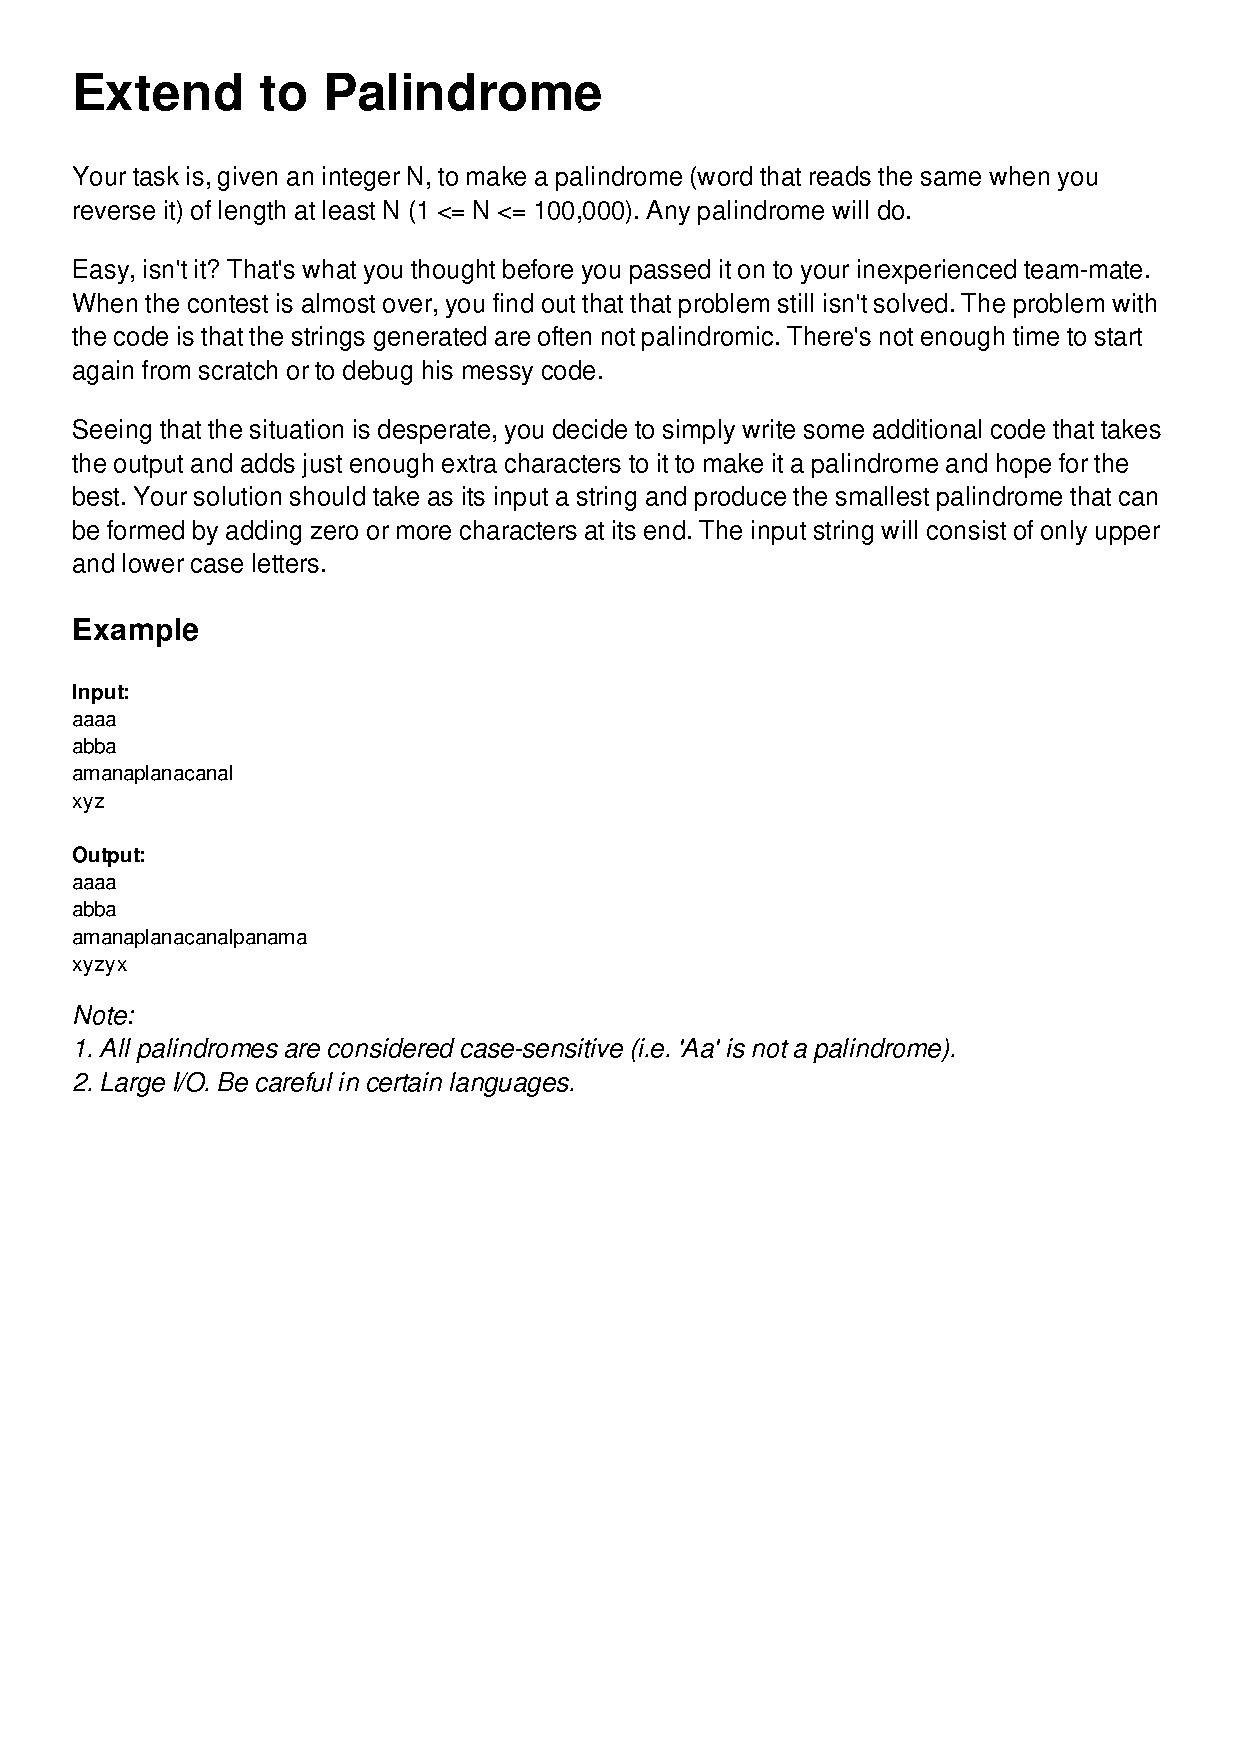
\includepdf[pages=-]{problemas/pdf/EPALIN.pdf}

\inputminted[linenos, frame=lines]{cpp}{problemas/cpp/EPALIN.cpp}
\pagebreak

\inputminted[linenos, frame=lines]{haskell}{problemas/haskell/EPALIN.hs}
\pagebreak

\subsection{Encontrar todas las ocurrencias de un patrón en un texto}
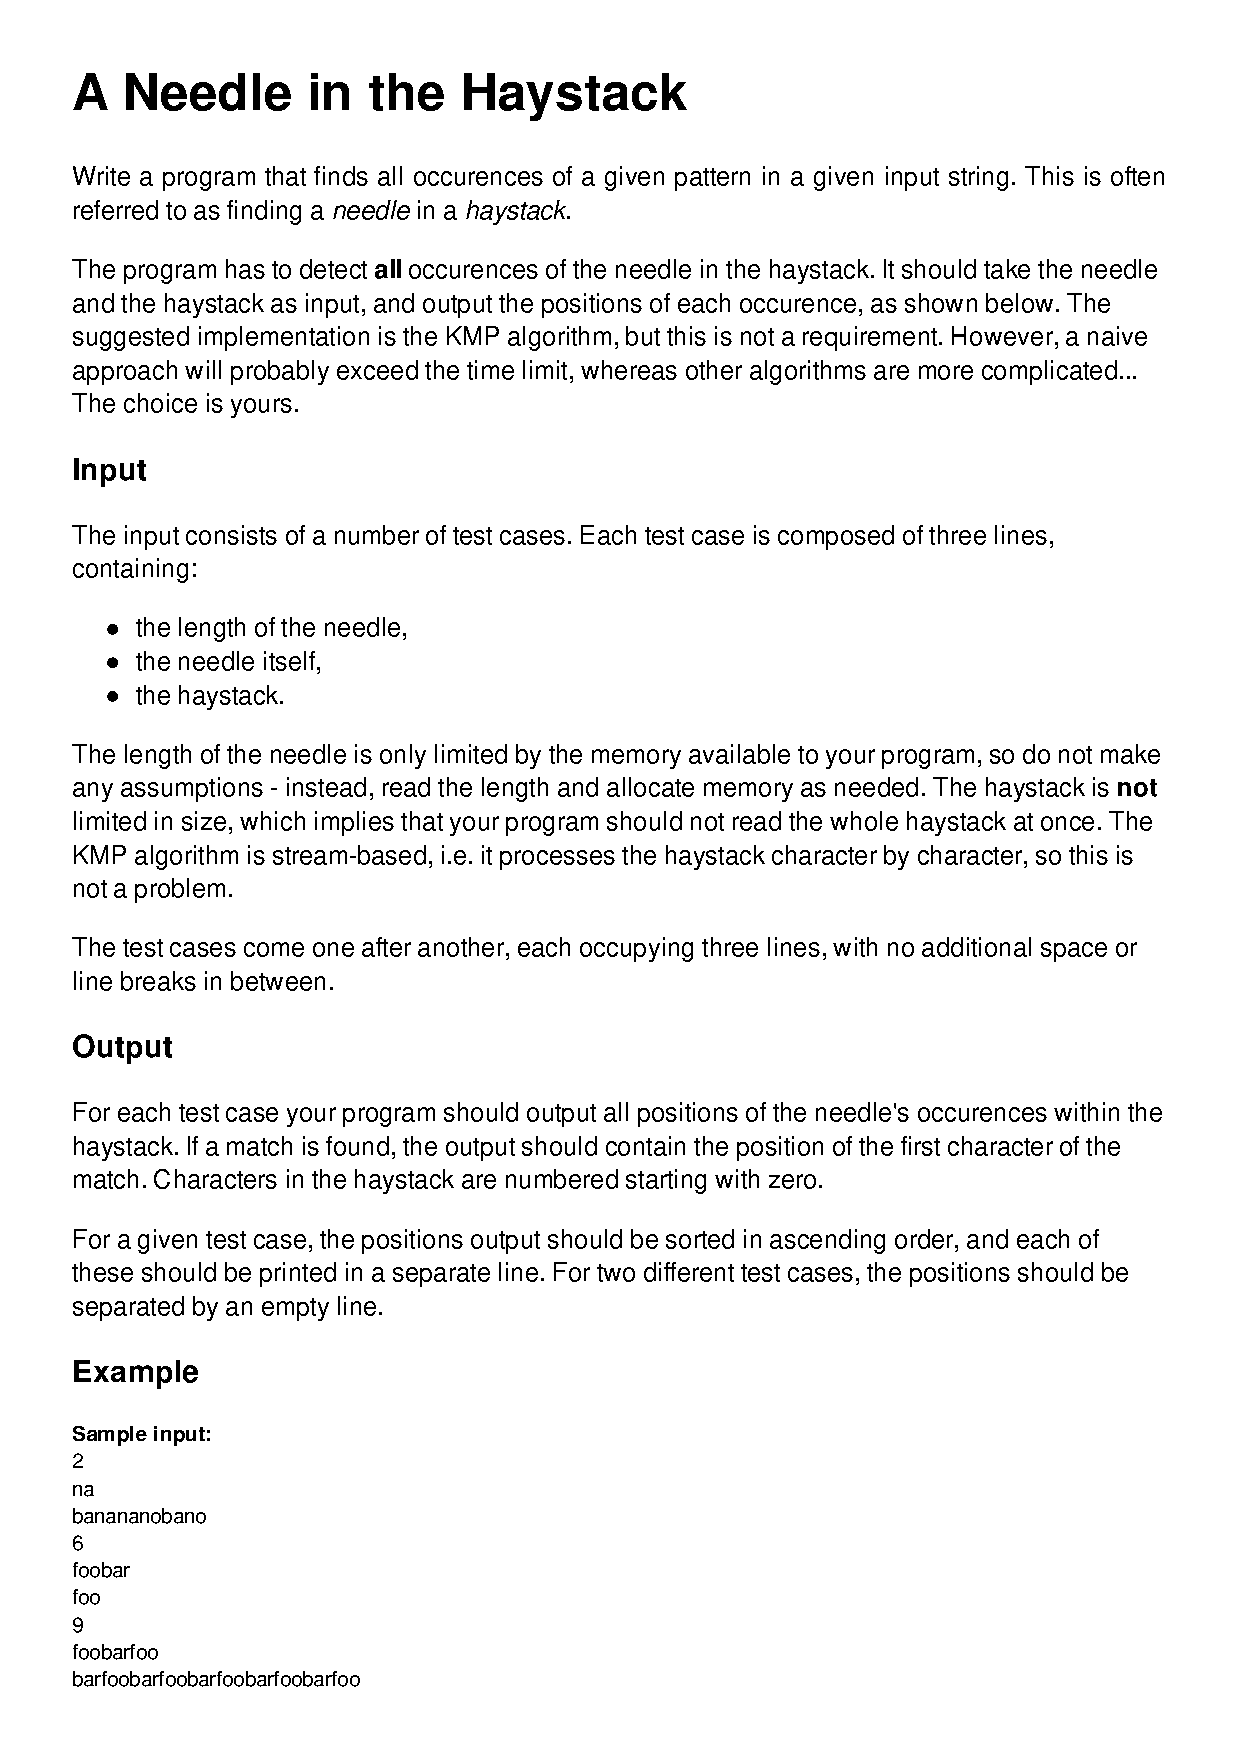
\includepdf[pages=-]{problemas/pdf/NHAY.pdf}

\inputminted[linenos, frame=lines]{cpp}{problemas/cpp/NHAY.cpp}
\pagebreak

\inputminted[linenos, frame=lines]{haskell}{problemas/haskell/NHAY.hs}
\pagebreak

% TODO: Chane y justifico esto el <$> https://ro-che.info/articles/2019-07-22-associativity-of-fmap

